\documentclass[10pt,a4paper]{article}
\usepackage[T1]{fontenc}
\usepackage[brazil]{babel}
\usepackage[utf8]{inputenc}


\usepackage{ae,aecompl}
\usepackage{pslatex}
\usepackage{epsfig}
\usepackage{geometry}
\usepackage{url}
\usepackage{textcomp}
\usepackage{ae}
\usepackage{subfig}
\usepackage{indentfirst}
\usepackage{textcomp}
\usepackage{color}
\usepackage{setspace}
\usepackage{verbatim}
\usepackage{amsmath}
\usepackage{enumitem}


% Gráficos
\usepackage{pgfplots}
\pgfplotsset{compat=1.3}
\usepgfplotslibrary{groupplots}

%  ABACO -- Conjunto de macros para desenhar o 'abaco

%  Desenho original de Hans Liesenberg

%  Macros de Tomasz Kowaltowski

%  DCC -- IMECC -- UNICAMP

%  Mar,co de 1988  --  Vers~ao 1.0

% Ajustado para LaTeX da SUN -- Mar,co de 1991

% ---------------------------------------------------------

%  Chamada:   \ABACO{d1}{d2}{d3}{d4}{esc}
%             com:  di's -- os quatro d'igitos;
%	           esc  -- fator de escala

% ---------------------------------------------------------

%  DEFINI,C~OES AUXILIARES

% ---------------------------------------------------------


%  Forma o d'igito pequeno (0 ou 1)

\newcommand{\ABACODP}[1]{%
%
\thicklines
%    
\begin{picture}(8,0)
    \ifcase#1{   %  caso 0
       \put(0,0)    {\line(1,0){4}}
       \multiput(5,0)(2,0){2}{\oval(2,4)}}
    \or{         %  caso 1
       \put(2,0)    {\line(1,0){4}}
       \multiput(1,0)(6,0){2}{\oval(2,4)}}
    \fi
\end{picture}
    } % \ABACODP

% Forma o d'igito grande (0 a 4)

\newcommand{\ABACODG}[1]{%
%
\thicklines
%    
\begin{picture}(14,0)
    \ifcase#1{   % caso 0
       \multiput(1,0)(2,0){5}{\oval(2,4)}}
       \put(10,0)   {\line(1,0){4}}
    \or{         % caso 1
       \multiput(1,0)(2,0){4}{\oval(2,4)}}
       \put(8,0)   {\line(1,0){4}}
       \put(13,0)   {\oval(2,4)}
    \or{         % caso 2
       \multiput(1,0)(2,0){3}{\oval(2,4)}
       \put(6,0)   {\line(1,0){4}}
       \multiput(11,0)(2,0){2}{\oval(2,4)}}
    \or{         % caso 3
       \multiput(1,0)(2,0){2}{\oval(2,4)}
       \put(4,0)   {\line(1,0){4}}
       \multiput(9,0)(2,0){3}{\oval(2,4)}}
    \or{         % caso 4
       \put(1,0)  {\oval(2,4)}}
       \put(2,0)   {\line(1,0){4}}
       \multiput(7,0)(2,0){4}{\oval(2,4)}
    \fi
\end{picture}
    } % \ABACODG
       
% Forma um d'igito (0 a 9)

\newcommand{\ABACOD}[1]{%
%
    \ifnum#1>9
       \errmessage{#1: Argumento invalido para ABACO}
    \fi
    \ifnum#1<0
       \errmessage{#1: Argumento invalido para ABACO}
    \fi
%
\begin{picture}(24,0)
%    
    \ifnum#1<5
       \put(16,0) {\ABACODP{0}}
    \else   
       \put(16,0) {\ABACODP{1}}
    \fi
%    
    \ifnum#1<5
       \put(0,0)  {\ABACODG{#1}}
    \else
       \ifcase#1\or \or \or \or
          \or  \put(0,0)  {\ABACODG{0}}
          \or  \put(0,0)  {\ABACODG{1}}
          \or  \put(0,0)  {\ABACODG{2}}
          \or  \put(0,0)  {\ABACODG{3}}
          \or  \put(0,0)  {\ABACODG{4}}
       \fi
    \fi   
\end{picture}
    } % \ABACOD
    
% -------------------------------------------------

%  DEFINI,C~AO PRINCIPAL
    
\newcommand{\ABACO}[5]{%
    \setlength{\unitlength}{#5mm}
%
    \thinlines
%   
\begin{picture}(28,25)
%   
% moldura
%
% externa
%
        \put(0,0)            {\line(0,1){25}}
        \put(0,0)            {\line(1,0){28}}
        \put(28,0)           {\line(0,1){25}}
        \put(0,25)           {\line(1,0){28}}
% interna
        \put(2,2)            {\line(0,1){21}}
	\put(26,2)           {\line(0,1){21}}
	\put(16,2)           {\line(0,1){21}}
	\put(18,2)           {\line(0,1){21}}
	\put(2,2)            {\line(1,0){14}}
	\put(16,2)           {\line(1,-1){1}}
	\put(17,1)           {\line(1,1){1}}
	\put(18,2)           {\line(1,0){8}}
	\put(2,23)           {\line(1,0){14}}
	\put(16,23)          {\line(1,1){1}}
	\put(17,24)          {\line(1,-1){1}}
	\put(18,23)          {\line(1,0){8}}
	\put(0,0)            {\line(1,1){2}}
	\put(0,25)           {\line(1,-1){2}}
	\put(28,0)           {\line(-1,1){2}}
	\put(28,25)          {\line(-1,-1){2}}
%
%   
% d'igitos
%
%   
       \put(2,20)  {\ABACOD{#1}}
       \put(2,15)  {\ABACOD{#2}}
       \put(2,10)  {\ABACOD{#3}}
       \put(2,5)   {\ABACOD{#4}}
%      
\end{picture}
    } % \ABACO
    
 

\renewcommand{\labelenumi}{\arabic{enumi}.}
\renewcommand{\labelenumii}{\arabic{enumi}. \arabic{enumii}}

\onehalfspacing
\begin{document}

% CAPA
\thispagestyle{empty}

\begin{minipage}[h]{0.10\linewidth}
  \ABACO{1}{9}{6}{9}{0.5} 
\end{minipage}
\begin{minipage}[h!]{0.7\linewidth}
  \vspace*{\fill}
  \centering
  {\large \textbf{UNIVERSIDADE~ESTADUAL~DE~CAMPINAS}}\\ 
  {\large INSTITUTO~DE~COMPUTAÇÃO}                   
  \vspace*{\fill} 
\end{minipage}
\\\vspace{0.5cm}

\begin{center} 
  \rule{11.0cm}{0.4pt}\vspace*{-\baselineskip}\vspace{-2.0pt}
  \rule{11.0cm}{1.6pt} \vspace*{-\baselineskip}
  {\Large \textsc{Reconhecimento de faces em redes sociais}}\vspace{3.2pt}
  \rule{11.0cm}{0.4pt}\vspace*{-\baselineskip}\vspace{3.2pt} \rule{11.0cm}{1.6pt}\\
  {\textsl{Proposta de projeto}}
  \\\vspace{1cm}
  \begin{tabular}{ll}
    Carlos Eduardo Rosa Machado & \textbf{RA}: 059582\\
    \multicolumn{2}{c}{\small \emph ra059582@students.ic.unicamp.br}  \\
    Douglas Alves Germano        & \textbf{RA}: 060210\\
    \multicolumn{2}{c}{\small \emph ra060210@students.ic.unicamp.br } \\
    Tiago Chedraoui Silva        & \textbf{RA}: 082941\\
    \multicolumn{2}{c}{\small \emph ra082941@students.ic.unicamp.br} \\
  \end{tabular}
\end{center}
\vspace{0.5cm}
\begin{abstract}

O Facebook é uma rede social gratuita, fundada em 2004, e atualmente possui mais de 700 milhões de usuários ativos. Muitas vezes, encontrar um usuário  a partir de informações não é algo fácil.
	
De forma a fornecer mais um método para encontrar um usuário, criou-se um sistema que, dado uma foto de entrada contendo uma face a ser procurada, retorna os perfis no Facebook com os rostos mais semelhantes ao objetivo dentre os amigos de amigos do usuário.
	
Apesar da dificuldade de se comparar faces, aplicando-se o PCA, encontrou-se sempre o usuário correto quando a foto de entrada no sistema era igual à foto de perfil utilizada e, para fotos distintas, apenas alguns usuários foram encontrados corretamente.
\end{abstract}

\tableofcontents
\newpage 
%\doublespacing

\section{Introdução e Motivação}

	Rede social é uma estrutura composta por indivíduos ou organizações, chamados de nós, que se conectam por um ou vários tipos de relações, tais como amizade, parentesco, interesses em comum, entre outras.
	
	O Facebook é uma rede social gratuita, fundada em 2004, e atualmente possui mais de 700 milhões de usuários ativos.

	Qualquer pessoa pode ter um perfil no Facebook, tornando-se um usuário do sistema. Para criar um perfil, ela deve fornecer informações pessoais como nome, localização, endereço eletrônico, e outras que desejar. Entre as opções, o usuário pode também fornecer uma foto para ser mostrada no perfil, que qualquer outro usuário terá acesso irrestrito para visualizá-la. Mesmo sem ter controle sobre a sua foto de perfil, esta é uma prática bastante utilizada pela maioria dos usuários, pois proporciona fácil reconhecimento para outros usuários. Além disso, o usuário pode colocar outras fotos pessoais, para as quais controlará o acesso, deixando restrito, por exemplo, apenas para aqueles que fazem parte da sua rede de relacionamentos no sistema.

	Pelo próprio intuito da rede, um usuário cadastrado quer se conectar e se relacionar virtualmente com as pessoas que conhece, ou até mesmo conhecer pessoas novas, quando algum interesse mútuo ocorre.

	Desta forma, o Facebook tem algumas ferramentas à disposição dos usuários, que permitem que pessoas sejam encontradas por outras usando alguma informação, tal como nome, endereço eletrônico ou endereço físico.

	Por isso, a ambição do projeto está em criar uma nova ferramenta, um novo meio para que as pessoas se encontrem e se conheçam. Pois, apesar do Facebook ter bons buscadores que encontram facilmente um usuário, precisamos sempre ter alguma informação pessoal, que podemos não saber ou não conseguir obter rapidamente. Contudo, podemos ter uma foto, e é neste caso que entra a nossa proposta de solução: buscar um perfil dado uma foto.
%\newpage
\section{O problema}

	Participar ativamente de uma rede social, tal qual o Facebook, está muito ligado em encontrar seus amigos online e fazer novos amigos, para assim trocar mensagens com os usuários, participar de eventos, estar presente em grupos, entre outras possibilidades. Por conseguinte, o problema está em conectar estes usuários, de modo que amigos recentes ou velhos amigos possam ser encontrados facilmente.

	É esperado que uma pessoa saiba, ou tenha anotado em algum lugar, informações básicas sobre seus amigos. Porém, nem sempre nos recordamos ou temos estes dados em mãos. Por exemplo, você acabou de conhecer uma pessoa, que por falta de tempo ou por distração, não perguntou o nome dela. Mas, como estavam numa festa e você tirou diversas fotos, acabou reconhecendo ela em uma das fotos. Assim, com as atuais ferramentas que o Facebook disponibiliza, você não seria capaz de encontrá-la facilmente, pois não sabe nada sobre a pessoa.

A proposta deste projeto é incluir uma ferramenta diferente, que não precisa de qualquer tipo de informação sobre o indivíduo, mas que seja capaz de encontrá-lo por comparação entre a imagem alvo, esta que você possui na sua câmera, com as imagens dos perfis dos usuários.

	Ou seja, o usuário fornece a foto com o rosto da pessoa que deseja buscar, o sistema varre a rede procurando as imagens mais semelhantes, e retorna os perfis que contêm os rostos mais parecidos, e eventualmente, o perfil correto do usuário buscado.

	De início, surgem dois problemas: encontrar uma face a partir de uma imagem e encontrar esta face em outras imagens. Assumindo que temos uma ferramenta capaz de reconhecer as características de um ser humano e recortar seu rosto, e outra que faça a comparação das faces detectadas, surge um problema bônus: a imensa quantidade de usuários cadastrados no Facebook.

	São centenas de milhões de pessoas ativas especificamente no Facebook, e portanto, fazer a comparação entre todos estes usuários em tempo razoável é uma outra dificuldade que enfrentamos.

	Deste modo, este projeto se propõe a fornecer um novo meio de encontrar usuários na rede utilizando apenas uma foto, mas que dê algum resultado, seja ele de sucesso ou fracasso, em um tempo hábil, mantendo a satisfação do cliente.

	Existem outros problemas com os quais lidaremos, mas que não
        temos muito o que fazer para saná-los, tais como: perfil
        criado sem foto ou que a foto não seja da pessoa, imagens
        ruins, ou então que não contenha um rosto, e etc.

\section{Solução proposta}
A abordagem tomada foi de criar um aplicativo externo ao Facebook, que utiliza das formas de conexões desenvolvidas e publicadas pela empresa, para interagir e manipular os dados necessários ao nosso projeto.
\subsection*{Definição do espaço:}

	A primeira precaução do grupo foi definir o espaço de busca do algoritmo. Dado que o Facebook registra em torno de 700 milhões de usuários ativos no sistema, fazer a comparação entre todos e retornar uma resposta adequada seria improvável, pois algoritmos semelhantes, como o do Picasa, demora 6 dias para comparar 50 mil fotos, tempo totalmente fora do esperado pelo usuário.

	Portanto, partimos da premissa que a pessoa buscada talvez
        seja um amigo de um amigo do usuário e nos limitamos nesta
        fronteira. De acordo com estudos realizados, um usuário médio
        tem em torno de 130 amigos na rede. Logo, estaríamos nos
        propondo a realizar a busca por 16900 usuários (130 x 130) no
        caso médio. Esta abordagem nos pareceu bastante favorável,
        para um retorno satisfatório em tempo adequado.

\subsection*{Graph API:}
O Facebook disponibiliza uma plataforma de desenvolvimento para qualquer pessoa que esteja interessada em iniciar um programa e utilizar as informações contidas nos perfis dos usuários. Vale ressaltar que nem todos os dados pessoais são públicos, a menos que o usuário habilite para que sejam. Entretanto, ao menos a foto do perfil, ponto de interesse do projeto, será visível a qualquer um.

	Toda informação está no que é chamado de grafo social, onde qualquer coisa é um nó, com identificador único, e possui relações com outros nós. Por exemplo, um usuário X é um nó e está conectado a outro usuário Y, também nó, por uma relação de amizade. São nós: usuários, eventos, fotos, páginas etc. E são conexões: amizade, participação em eventos, marcação em fotos e outros.

	Tudo isto está disposto numa arquitetura de JSON facilmente entendida. Um JSON é composto por uma propriedade e seu valor. Ou seja, para um usuário teremos, por exemplo, a propriedade nome e o seu valor, seu nome.

\subsection*{PCA:}

	PCA (Principal Component Analysis) é um método da família de “análise de dados”, que consiste em transformar variáveis correlacionadas em novas variáveis independentes umas das outras. Essas novas variáveis são chamadas de “componentes principais”, ou eixos. Elas permitem reduzir a informação a um número de variáveis mais limitado que o inicial.

	Encontrando os componentes principais da distribuição das faces, ou os autovetores da matriz de covariância do conjunto das imagens (tratando cada imagem como um ponto num espaço de dimensão alta), obtemos as chamadas autofaces.

	As autofaces resultantes podem ser pensadas como um conjunto de características que, juntas, formam a base do espaço das faces. Cada rosto, pode ser, então, projetado sobre esses vetores, de modo que cada imagem possa ser armazenada como uma simples combinação linear.

Porém, devido a algumas limitações do PCA, precisamos fazer alguns tratamento nas imagens.

	O primeiro tratamento é simples: apenas transformamos as fotos da escala RGB em escala de tons de cinza. Para reduzirmos a interferência das tonalidades nos resultados.

	Outro procedimento básico é deixar todas as imagens no mesmo tamanho. Faz mais sentido comparar fotos de tamanhos idênticos do que fotos muito maiores do que outras, pois o PCA é variante à escala.

	E um problema menos intuitivo é a exposição das imagens à iluminação. O resultado final é muito atrapalhado por comparação entre fotos com tons de luz diferentes. Por isto, aplicamos uma equalização do histograma, reduzindo a dependência da iluminação.


Para o reconhecimento, projeta-se uma nova imagem nesse mesmo espaço formado pelas autofaces e, então, classifica-se a face comparando sua posição no espaço com a posição dos outros rostos, conhecidos.

Abaixo segue a explicação mais detalhada do processo.
\subsubsection*{Treinamento:}
Sejam $\Gamma_1, \Gamma_2, \Gamma_3, \ldots, \Gamma_m$ as imagens de faces para treinamento. A face média é definida por {$\Psi  =\frac{1}{M}* \sum_{i=1}^m\Gamma_i$}. Cada face difere da média pelo vetor {$\Phi_i = \Gamma_i - \Psi$}.

Queremos, através do PCA, obter M vetores ortonormais, $u_n$, que melhor descrevem a distribuição dos dados. O k-ésimo vetor é escolhido de tal forma que

\begin{equation}
  \lambda_{k}=\frac{1}{M}\sum_{n=1}^{M}(u_k^T\Phi_n)^2
\end{equation}

é um máximo, sujeito a

\begin{equation}
  u_l^Tu_k=\delta_{lk}=\left \{
    \begin{array}{l l}
      1, & \quad \text{se $l=k$} \\
      0, & \quad \text{caso contrário}\\
    \end{array}
  \right.
\end{equation}

Os vetores $u_k$ e escalares $\lambda_k$ são os autovalores e autovetores da matriz de covariância

\begin{equation}
  C=\frac{1}{M}\sum_{n=1}^{M}(\Phi_n\Phi_n^T)= AA^T
\end{equation}

onde $A = [ \Phi_1 \Phi_2 \ldots \Phi_m ]$, matriz na qual cada coluna é uma das faces de treinamento. Supondo que cada imagem de face é composta por NxN pixels, esta matriz C será, então, $N^2 \times N^2$. Todavia, se o número de rostos for bem menor do que o tamanho de cada foto ($M \ll N$), podemos simplificar os cálculos, se considerarmos a matriz $A^TA$:

\begin{equation}
  A^TAv_i=\mu_iv_i
\end{equation}

Nesse caso, $\mu_i$ e $v_i$ são, respectivamente, os autovalores e autovetores de $A^TA$. Multiplicando ambos os lados por A, temos:

\begin{equation}
  AA^TAv_i=\mu_iAv_i
\end{equation}

De onde vemos que $Av_i$ são os autovetores da matriz original $C = AA^T$.

Se, por exemplo, temos 300 imagens, cada uma com 100 x 100 pixels, teremos, então, que resolver uma matriz de $9*10^4$ elementos, ao invés de $10^8$, o que torna o treinamento ordens de grandeza mais rápido.

\subsubsection*{Reconhecimento:}

Com os autovetores obtidos, temos nosso “espaço de faces”. Vale ressaltar que nem todos os autovetores são necessários para uma boa representação do conjunto de imagens. Assim, escolhemos apenas um subconjunto de tamanho M’ desses vetores (mais especificamente os que possuem os maiores autovalores associados) para descrever o espaço.

Para reconhecimento de faces, precisamos, primeiro, classificar cada indivíduo conhecido. Para isso, projetamos cada imagem de face conhecida em nosso espaço de faces, obtendo o vetor de classe $\Omega_k^T = [ \omega_1, \omega_2, \ldots,\omega_{M'} ]$, onde:

\begin{equation}
  \omega_k=u_k^T(\Gamma-\Psi)
\end{equation}

Em seguida, dada uma face de entrada que queremos reconhecer, basta projetá-la também no espaço, obtendo o vetor $\Omega$. Calculamos, então, a distância euclidiana dessa classe às classes reconhecidas:

\begin{equation}
  \epsilon_k^2=\|\Omega-\Omega_k\|^2
\end{equation}

Basta, enfim, encontrar a classe c tal que o mínimo das distâncias $\epsilon_c$ é menor do que um limiar escolhido $\theta_k$.

\subsection*{Desenvolvimento:}
	Com as informações obtidas do Graph API, e conhecendo sua estrutura formada por JSON, optamos por utilizar Python para o desenvolvimento. Mostrou-se interessante num primeiro momento, pela grande facilidade de realizar conexões com o Facebook e de manipular as respostas recebidas em formato JSON.

	Inicialmente, escrevemos nosso módulo “facebook” (em facebook.py), no qual colocamos todas as funções que se comunicam com o grafo social. Entre elas, temos as genéricas get\underline{ }user\underline{ }connection e batch\underline{ }request. A primeira realiza um simples GET de um único elemento do grafo, tal como nome, lista de amigos ou lista de fotos de um único usuário; a segunda, por sua vez, mostrou-se necessária para obtermos mais informações em uma única conexão com o servidor: pode-se agrupar no máximo 20 requisições simples em um único pacote, e esses dados são obtidos através de um só POST. As demais funções apenas usam essas duas para obter todos os dados necessários para nosso sistema (amigos, foto de perfil e fotos marcadas, por exemplo).

	Em seguida, criamos o módulo “eigenfaces”, que utiliza a biblioteca Numpy (para operações otimizadas em vetores e matrizes) no cálculo da face média, dos autovalores e autovetores representando o espaço de faces, da projeção de uma imagem nesse espaço e das distâncias de uma face a todas as classes conhecidas.

	Para o próximo problema, a detecção de faces, a intenção inicial era fazer a implementação utilizando C++, devido à boa documentação do pacote OpenCV disponível. Mas, desde a versão mais nova (2.2) da biblioteca, uma interface Python que cobre todas as funções C++ também é oferecida. Optamos, então, por trabalhar com apenas uma linguagem nesse momento de implementação do primeiro protótipo.

	Então, criamos as funções auxiliares detect\underline{ }image\underline{ }faces, que
        retorna a posição de faces em uma imagem; crop\underline{ }face\underline{ }image, que
        recorta um retângulo de uma imagem; crop\underline{ }tagged\underline{ }photo, que,
        dado um link e uma tag retornados por get\underline{ }user\underline{ }tags (do módulo
        “facebook”), obtém a imagem e recorta apenas o local onde o
        usuário está possivelmente marcado; save\underline{ }user\underline{ }face, que, dado
        um número de usuário, tenta obter uma imagem de seu rosto; e
        iniciamos nosso sistema “facefinder”, que realiza os seguintes
        passos para uma imagem de entrada $\Gamma$:


\begin{enumerate}
	\item Cria diretórios “pictures”, que guarda as fotos originais baixadas de cada usuário, e “faces”, que guarda apenas as faces recortadas e ajustadas dos mesmos;
	\item Obtém a lista dos amigos de amigos do usuário;
	\item Para cada usuário na lista, lança uma thread iniciando
          em save\underline{ }user\underline{ }face, que
          especificamente:
          \begin{enumerate}
          \item Não faz nada se a face do usuário já está em disco;
          \item Se nenhuma foto do usuário está presente, baixa a
            foto de perfil;	
          \item Procura uma face na imagem corrente, preprocessando e retornando-a se for encontrada;
          \item Se face não foi encontrada, pega uma foto em que
            o usuário foi marcado e repete a partir de 3.3;
          \end{enumerate}
	\item Carrega espaço de faces se um existir OU obtém um espaço de faces a partir de imagens pré-determinadas numa pasta “training” OU obtém um espaço de faces a partir das obtidas baixadas por 3;
	\item Projeta $\Gamma$ e as faces obtidas em 4 nesse espaço;
	\item Encotra as classes mais próximas de $\Gamma$.
\end{enumerate}

	Por fim, utilizamos o pacote Pygame, que oferece módulos para tratar eventos de periféricos e para gerenciar janelas gráficas, com o objetivo de criar uma interface de fácil utilização para o usuário, descrita no próximo tópico.

\subsection*{Interface:}
	O usuário precisa fornecer uma foto da pessoa que ele quer procurar. O programa tenta detectar rostos na imagem, e destaca cada face utilizando retângulos. Basta então, que o rosto desejado seja selecionado (ver figura 1).

\begin{figure}[h!]
  \begin{center}
    \includegraphics[scale=0.3]{Screenshot-Face}
    \caption{Seleção de faces}
  \end{center}
\end{figure}

Caso nenhuma face seja detectada automaticamente, o usuário tem a possibilidade de designar a face através de um retângulo ajustável (ver figura 2).

\begin{figure}[h!]
  \begin{center}
    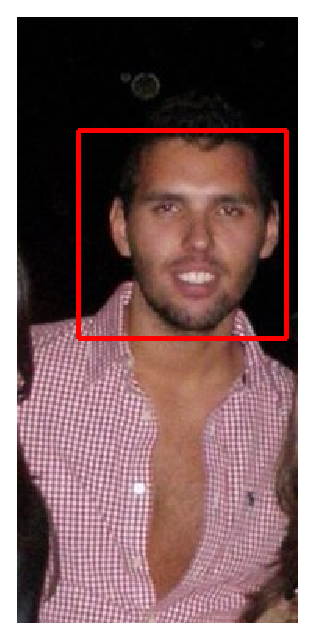
\includegraphics[scale=0.4]{samephoto}
    \caption{ Seleção da face na foto fornecida}
  \end{center}
\end{figure}

Após a seleção da face, o usuário aguarda um breve instante, até que o
aplicativo faça a comparação e busca, e assim o resultado será
mostrado numa janela. Optamos por mostrar as 6 pessoas com rostos mais
parecidos ao rosto alvo (ver figura 3).

\begin{figure}[h!]
    \begin{center}
      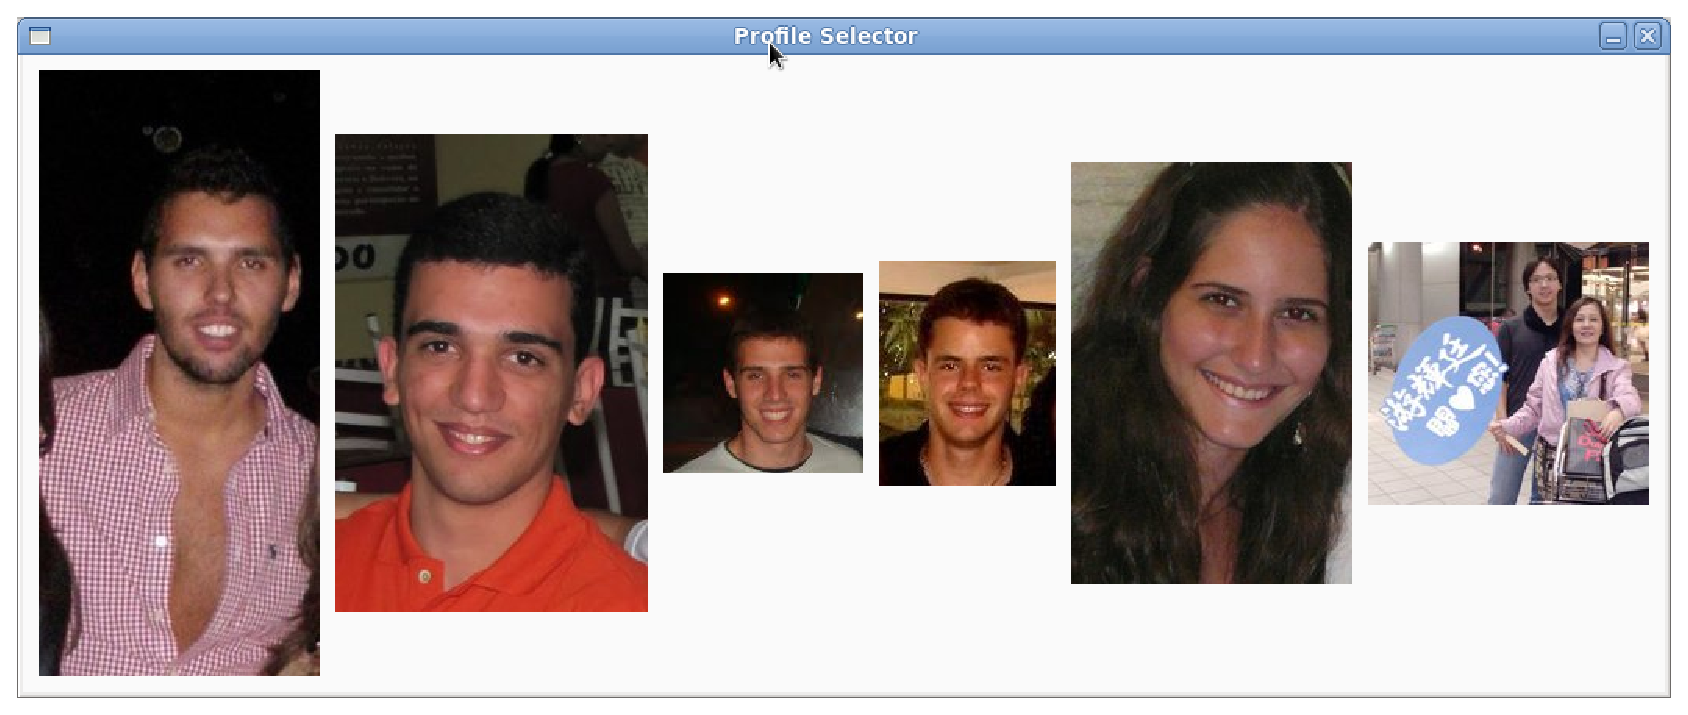
\includegraphics[scale=0.4]{6maisproximos}
      \caption{Faces mais próximas}
    \end{center}
  \end{figure}


O usuário, então, escolhe qual dos perfis mostrados é a pessoa que está procurando. No caso em que o perfil é corretamente identificado, o usuário pode simplesmente clicar sobre a foto desejada e ele será redirecionado para a página dessa pessoa no Facebook.

No caso de fracasso da busca, o usuário não encontrará o perfil correto entre os 6 mais parecidos, seja porque a pessoa não possui um perfil ou porque o algoritmo não conseguiu encontrar uma foto semelhante. Neste caso, basta fechar a janela.

  

\section{Exprerimentos}%OK

Ao longo do desenvolvimento do projeto, fizemos algumas medições para encontrarmos
rapidamente qual seriam os possíveis gargalos do aplicativo. E encontramos problemas na definição do número de usuários que seriam utilizados na busca, no ajuste da ferramenta que realiza detecção de faces e no próprio algoritmo do PCA.

\subsubsection*{Definição de espaço}
	
Como descrito, a primeira abordagem que adotamos foi definir o espaço no qual iríamos fazer as buscas. Para isto, implementamos o algoritmo e executamos algumas vezes.

	A primeira versão baixava fotos de perfis do Facebook sequencialmente, o que causou um certo espanto, pois o tempo gasto para baixar 2000 fotos era de aproximadamente 70 minutos. Completamente inviável para a nossa proposta de realizar a busca completa em tempo hábil.

	Obviamente, precisávamos fazer este processo em paralelo. E assim, utilizando threads e requisições em lote, o tempo baixou de 70 minutos para 1 minuto e meio, também para 2000 fotos. De modo que utilizando o usuário médio, com 130 amigos, seria razoável realizar a busca apenas entre os amigos de seus amigos, o que nos daria aproximadamente 17000 pessoas. Ou seja, por volta de 13 minutos para obter as fotos.
\subsubsection*{Detecção de faces} 
	Com as fotos já em disco, precisávamos filtrá-las retirando elementos que interferissem mais do que desejaríamos no resultado da busca. Por isto, recortamos e utilizamos apenas os rostos.

	Nesta etapa, o foco mudou do tempo gasto para qualidade do resultado. Pois no caso da definição de espaço, estávamos interessados em diminuir o intervalo de tempo necessário para baixar fotos, e na detecção de faces estamos preocupados com a qualidade das fotos recortadas. Isto é, precisamos encontrar o maior número de faces, mas não queremos encontrar imagens que não sejam faces.

	Inicialmente, obtínhamos somente a foto de perfil de cada usuário. Nessa abordagem, o número de faces recortadas pelo algoritmo representava 57\% do total de fotos baixadas.

	Conseguimos melhorar este resultado tentando localizar rostos em outras fotos (marcadas), além da foto de perfil. Com esse método, chegamos a 86\% de faces extraídas.

	Porém, um outro dado interessante é quantas imagens tinham realmente rostos. Em torno de 15\% das “faces” recortadas eram falsos positivos, podendo ser desenhos, animais, ou outras formas semelhantes.

	Considerando os dois resultados, nosso aplicativo obteve uma taxa de 73\% de acerto ao detectar e recortar rostos, o que nos pareceu muito bom, pois não conseguimos controlar as fotos dos usuários.
\subsubsection*{Reconhecimento}
	Após aplicar o algoritmo para encontrar os rostos, trabalharemos nesta etapa somente com as imagens geradas pelo recorte das faces detectadas no passo anterior. 

	Para tentar obter uma boa decomposição do espaço de faces em
        componentes principais, escolhemos para a fase de treinamento
        algumas fotos fixas, que consideramos melhores. Isto é,
        imagens obtidas de diversas execuções do sistema, sem
        elementos como óculos, chapéu, rostos inclinados, e outros.

\begin{figure}[h!]
  \begin{center}
    \includegraphics[scale=1.0]{avg}
    \caption{Face média para o conjunto de imagens utilizado}
  \end{center}
\end{figure}

\newpage
	Considerando tudo isto, trabalhamos com três resultados possíveis:

        \begin{enumerate}
	\item A foto fornecida é a mesma foto que foi utilizada pelo sistema para detectar a face do usuário (chamada, daqui pra frente, de origem). Nesse caso, o nosso algoritmo funcionou 100\% das vezes, retornando sempre o perfil do usuário buscado entre os 6 mais semelhantes. Vale ressaltar que só utilizamos para classificação os usuários que tiveram rostos devidamente encontrados em suas fotos de origem.


\begin{flushleft}
\begin{figure}[h!]
\begin{flushleft}
\subfloat[Seleção de face]{\includegraphics[scale=0.15]{davi-fs}
} \subfloat[Alvo]{\includegraphics[scale=0.6]{davi-target}} \subfloat[Fotos mais próximas]{\includegraphics[scale=0.3]{davi-ps}}
\caption{Foto igual a do perfil}
\par\end{flushleft}
\end{figure}
\par\end{flushleft}

\begin{table}[h!]
\begin{center}
\begin{tabular}{cc}
Distância & ID perfil \\
\hline
24.6135480676 & 1215224340\\
2574.39277549 & 100001873433028\\
2879.24733272 & 1764741129\\
2982.18618505 & 1042957106\\
3020.20152097 & 1791523169\\
3078.53580598 & 100000635998652
\end{tabular}
\end{center}
\end{table}



\begin{flushleft}
\begin{figure}[h!]
\begin{flushleft}
\subfloat[Seleção de face]{\includegraphics[scale=0.45]{por}
} \subfloat[Alvo]{\includegraphics[scale=0.6]{portg}} \subfloat[Fotos mais próximas]{\includegraphics[scale=0.4]{por2}}
\caption{Foto igual a do perfil}
\par\end{flushleft}
\end{figure}
\par\end{flushleft}

\begin{table}[h!]
\begin{center}
\begin{tabular}{cc}
Distância & ID perfil \\
\hline
60.2425391933 & 100000159379017\\
3629.41351482 & 100001749012330\\
3735.50400304 & 100001921657622\\
3877.18252151 & 1791523169\\
3882.86934524 & 100001397308579\\
3999.35526051 & 1215224340
\end{tabular}
\end{center}
\end{table}



	\item A foto alvo fornecida é uma foto "boa" e diferente da origem. Encontramos uma certa dificuldade nesse caso, pois podemos sofrer grande influência de elementos externos às fotos. Exemplo: o usuário faz poses diferentes nas fotos, inclinando-se ora para esquerda, ora para direita.


\begin{flushleft}
\begin{figure}[h!]
\begin{flushleft}
\subfloat[Seleção de face]{\includegraphics[scale=0.25]{medu}
} \subfloat[Alvo]{\includegraphics[scale=0.6]{medutg}} \subfloat[Fotos mais próximas]{\includegraphics[scale=0.3]{medu2}}
\caption{Foto diferente do perfil: Perfil correto encontrado}
\par\end{flushleft}
\end{figure}
\par\end{flushleft}

\vspace{-0.5cm}
\begin{table}[h!]
\begin{center}
\begin{tabular}{cc}
Distância & ID perfil \\
\hline
2602.09124834 & 1808007231\\
2662.35298832 & 100000152641021\\
2689.05046879 & 100001638709636\\
3159.89846074 & 1577056142\\
3287.69470265 & 100001739081454\\
3295.47052987 & 100000418692820
\end{tabular}
\end{center}
\end{table}


\begin{flushleft}
\begin{figure}[h!]
\begin{flushleft}
\subfloat[Seleção de face]{\includegraphics[scale=0.25]{kuni}
} \subfloat[Alvo]{\includegraphics[scale=0.6]{kunitg}} \subfloat[Fotos mais próximas]{\includegraphics[scale=0.3]{kuni2}}
\caption{Foto diferente do perfil: Perfil correto não encontrado}
\par\end{flushleft}
\end{figure}
\par\end{flushleft}


\begin{table}[h!]
\begin{center}
\begin{tabular}{cc}
Distância & ID perfil \\
\hline
4966.66383286 & 100001541135744\\
5262.51189874 & 100000471103949\\
5376.08766636 & 668787604\\
5482.40195199 & 1191854356\\
5516.23024307 & 100000159379017\\
5653.01049558 & 100000227946853
\end{tabular}
\end{center}
\end{table}

	\item A foto alvo fornecida é "boa", mas a foto de origem é "ruim" ou inexistente. Aqui, designamos vários casos por fotos "ruins": imagem com qualidade ruim, imagem rotacionada, rosto detectado é de animal ou desenho, entre outros. A taxa de acertos para esse caso será de 0\%, visto que esse usuário dificilmente será “classificado” no espaço de faces, impossibilitando a comparação.



\begin{flushleft}
\begin{figure}[h!]
\begin{flushleft}
\subfloat[Seleção de face]{\includegraphics[scale=0.25]{rocha}
} \subfloat[Alvo]{\includegraphics[scale=0.9]{rochatg}} \subfloat[Fotos mais próximas]{\includegraphics[scale=0.3]{rocha2}}
\caption{Foto sem perfil}
\par\end{flushleft}
\end{figure}
\par\end{flushleft}


\begin{table}[h!]
\begin{center}
\begin{tabular}{cc}
Distância & ID perfil \\
\hline
4632.66984794 & 100000159379017\\
4976.20171369 & 100000481558433\\
5019.12654823 & 100001364636243\\
5158.32148578 & 100000411131240\\
5246.54044531 & 100000471103949\\
5673.87138099 & 668787604
\end{tabular}
\end{center}
\end{table}

\end{enumerate}

\subsubsection*{Testes }

Por fim, realizamos um teste final rodando o programa a partir de 3 usuários diferentes. Para isso, escolhemos 100 usuários aleatoriamente que estão presentes nos conjuntos de amigos de amigos dos 3 usuários. Para os 100 usuários, baixamos suas fotos de perfil e uma foto aleatória em que foi marcado. Utilizamos, então, a ferramenta "facelector" em cada uma das fotos marcadas para recortar somente a face do usuário que nos interessa (o mesmo que teve sua foto de perfil baixada). A tabela abaixo indica quantas fotos e quantas faces foram utilizadas para classificação nos experimentos.

\begin{table}[h!]
\begin{center}
\caption{Número de faces e fotos para os usuários}
\begin{tabular}{ccc}
\hline
Usuário & n° fotos & n° faces \\
\hline
\hline
1 & 7200 & 4000 \\
2 & 3800 & 2200 \\
3 & 28900 & 15300 
\end{tabular}
\end{center}
\end{table}

Foram realizados quatro diferentes testes, nos quais as 100 faces recortadas foram usadas como entrada para o programa, alterando-se as fotos utilizadas no treinamento e a quantidade de autofaces mantidas: um teste com autovetores representando 75\% da energia e 370 faces "boas" escolhidas manualmente para treinamento, outro com 90\% e as mesmas faces "boas", outro com 75\% e 1000 faces escolhidas aleatoriamente para treinamento e, por fim, um com 90\% e as mesmas 1000 faces escolhidas aleatoriamente. Analisamos, em cada teste, qual seria a porcentagem Y de acerto ao retornar as X classes que o programa considerou as mais próximas da face alvo.

Fixando o conjunto de treinamento e variando o número de autofaces escolhidas, observamos que um maior número de autofaces tem maior porcentagem de acertos para um mesmo número X de classes mais próximas ao alvo. Mantendo fixo o número de autofaces e alterando o conjunto de treinamento, por sua vez, nos mostrou que as 1000 faces escolhidas aleatoriamente tiveram performance melhor do que as 370 faces "boas" (centralizadas, sem óculos e de rosto inteiro), escolhidas manualmente.

No gráfico abaixo, exibimos os resultados para os três diferentes usuários com fotos aleatórias para o treinamento e 75\% de energia. Para um usuário com mais amigos, apesar de ter mais chance da pessoa buscada estar no seu limite, a probabilidade de encontrá-lo é muito baixa. Já para usuários com menor número de amigos, acontece o inverso: menor número de pessoas buscadas e maior probabilidade de encontrá-lo, se ele estiver entre os buscados.

\begin{figure}
\begin{center}
\begin{tikzpicture}
\begin{axis}[
	x tick label style={
		/pgf/number format/1000 sep=},
	ylabel= Fotos encontradas em \%,
	enlargelimits=0.15,
	legend style={at={(0.5,-0.30)},
		anchor=north,legend columns=-1},
              nodes near coords,
	ybar,
        height=8cm,
        width=16cm,
	bar width=7pt,
        xlabel=Posição,
        xtick ={1, 2, 3, 4, 5, 6,7,8,9,10},
        xticklabels={1-10,11-50,51-100,101-200,201-300,301-500,501-1000,1001-2000,2001-3000,3001-Max},
        xticklabel style={rotate=90}
        ]

    \addplot  table[x=pos,y=num] {graf/tcs/75albar.txt};
    \addplot  table[x=pos,y=num] {graf/tcs/75albardoug.txt};
    \addplot  table[x=pos,y=num] {graf/tcs/75albarcar.txt};

\legend{Usu\'ario 1, Usu\'ario 2, Usu\'ario 3}
\end{axis}
\end{tikzpicture}
\end{center}
\caption{Fotos aleatórias para o treinamento e 75\% de energia}
\end{figure}

\section{Conclusões}

Apesar dos problemas encontrados, a solução proposta utilizando PCA
não atende razoavelmente as expectativas. O algoritmo tem performance
excelente quando a foto do perfil é exatamente a buscada, mas possui
um resultado ruim quando elas diferem.

	O aplicativo fica exposto a certas limitações que são inerentes ao problema. Para citar, há casos básicos como a pessoa não possuir perfil; casos em que não conseguimos encontrar um rosto na foto de perfil; e casos nos quais mesmo fazendo a busca por fotos de perfil atuais e fotos marcadas, o algoritmo não consegue encontrar semelhanças entre duas imagens com a mesma face. Neste último, geralmente as fotos possuem características incomuns, tais como rostos virados para lados opostos, iluminação ou contraste diferentes, entre outros elementos.

	Entretanto, essa implementação um tanto quanto “simples”, em um curto período de tempo, já foi suficiente para resolver parte do problema, o que é um convite para atacá-lo mais profundamente. Neste primeiro protótipo, nós focamos em obter uma solução que fosse rápida o bastante ao ser rodada do zero para um único usuário, isto é, que não demore muito ao ter que passar por todas as fases do programa (obtenção de amigos, obtenção de fotos, detecção de faces, análise dos componentes principais, classificação e reconhecimento da face). Assim, muitas de nossas escolhas foram feitas visando esse balanço.

	Porém, num próximo momento, de expansão do sistema, esse
        deverá servir um grande número de pedidos ao mesmo tempo, para
        um número cada vez maior de usuários. Para isto, modificações
        deverão ser feitas para torná-lo escalável e mais preciso. 

Listamos aqui, então, possíveis melhorias e rumos que podemos tomar
daqui pra frente:
\begin{itemize}
	\item Guardar localmente as listas de amigos obtidas;
	\item Guardar localmente mais de uma foto por usuário;
	\item Usar o máximo número possível de fotos diferentes de um usuário para classificá-lo;
	\item Classificar como rosto de usuário somente fotos nas quais apenas uma única face é detectada;
	\item Reduzir domínio a partir de informações adicionais sobre a pessoa buscada, como: sexo, etnia ou língua falada;
	\item Usar distâcia de Mahalanobis ao invés de distância Euclidiana;
	\item Usar outro método para reconhecimento de faces.
\end{itemize}
\vspace{-0.5cm}
% ******************************************************
% REFERENCIAS BIBLIOGRÁFICAS
% ******************************************************
% \section{Referências}
\bibliographystyle{plain}
\begin{small}
  \bibliography{referencias}
\end{small}


\end{document}